\chapter{Beyond Reinforcement Learning for Real World Robotic Visual Navigation}\label{ch:rl4rvsn}

\section{Offline Reinforcement Learning for Robotic Visual Navigation}\label{sec:offline_rl4rvsn}

\subsection{Introduction}\label{subsec:introduction_offnav}

The task of delivering Visual Semantic Navigation (\acrshort{vsn}) capabilities to real robots in the real world is still a challenge.
To teach robots how to navigate in indoor environments, the \acrshort{vsn} community has been using online reinforcement learning (RL) algorithms, which require querying environments to learn.
This is a problem because querying real environments is expensive and time-consuming, and querying simulated environments is not always a good proxy for real-world performance.
Offline RL~\cite{levine2020} can be a solution to these challenges by learning policies from a fixed dataset consisting in human demonstrations and their associated reward signals.
Therefore, in this work, we propose a novel approach to train \acrshort{vsn} agents without ever querying an environment, by leveraging on the Offline RL paradigm.
We call this approach \textbf{Off}line Visual Semantic \textbf{Nav}igation (OffNav).

Technically, we have implemented Implicit Q-Learning (IQL)~\cite{kostrikov2022offline} offline RL algorithm using the decentralized distributed philosophy of DD-PPO~\cite{wijmans2020} to create DD-IQL, a decentralized distributed version of IQL\@.
Our DD-IQL is trained against a fixed dataset containing thousands of human navigation experiences~\cite{ramrakhya2023}.
As depicted in Figure~\ref{fig:abstract_offnav}, we propose the OffNav approach, capable of efficiently learning the navigation policy required by a \acrshort{vsn} agent from human demonstrations.
Subsequently, these policies can be deployed across various scenarios, and if necessary, further refined through online RL for more specific tasks.

To demonstrate the capabilities of our implementation, we carried out a small analysis of its performance using different environments from HM3D dataset~\cite{Ramakrishnan2021HabitatMatterport3D}.
Preliminary results shows that our DD-IQL implementation is able to learn navigation policies effectively.
To the best of our knowledge, this is the first time that an offline RL algorithm is implemented for \acrshort{vsn}\@ and large environments, predicting actions directly from raw input observations.

\begin{figure}
    \centering
    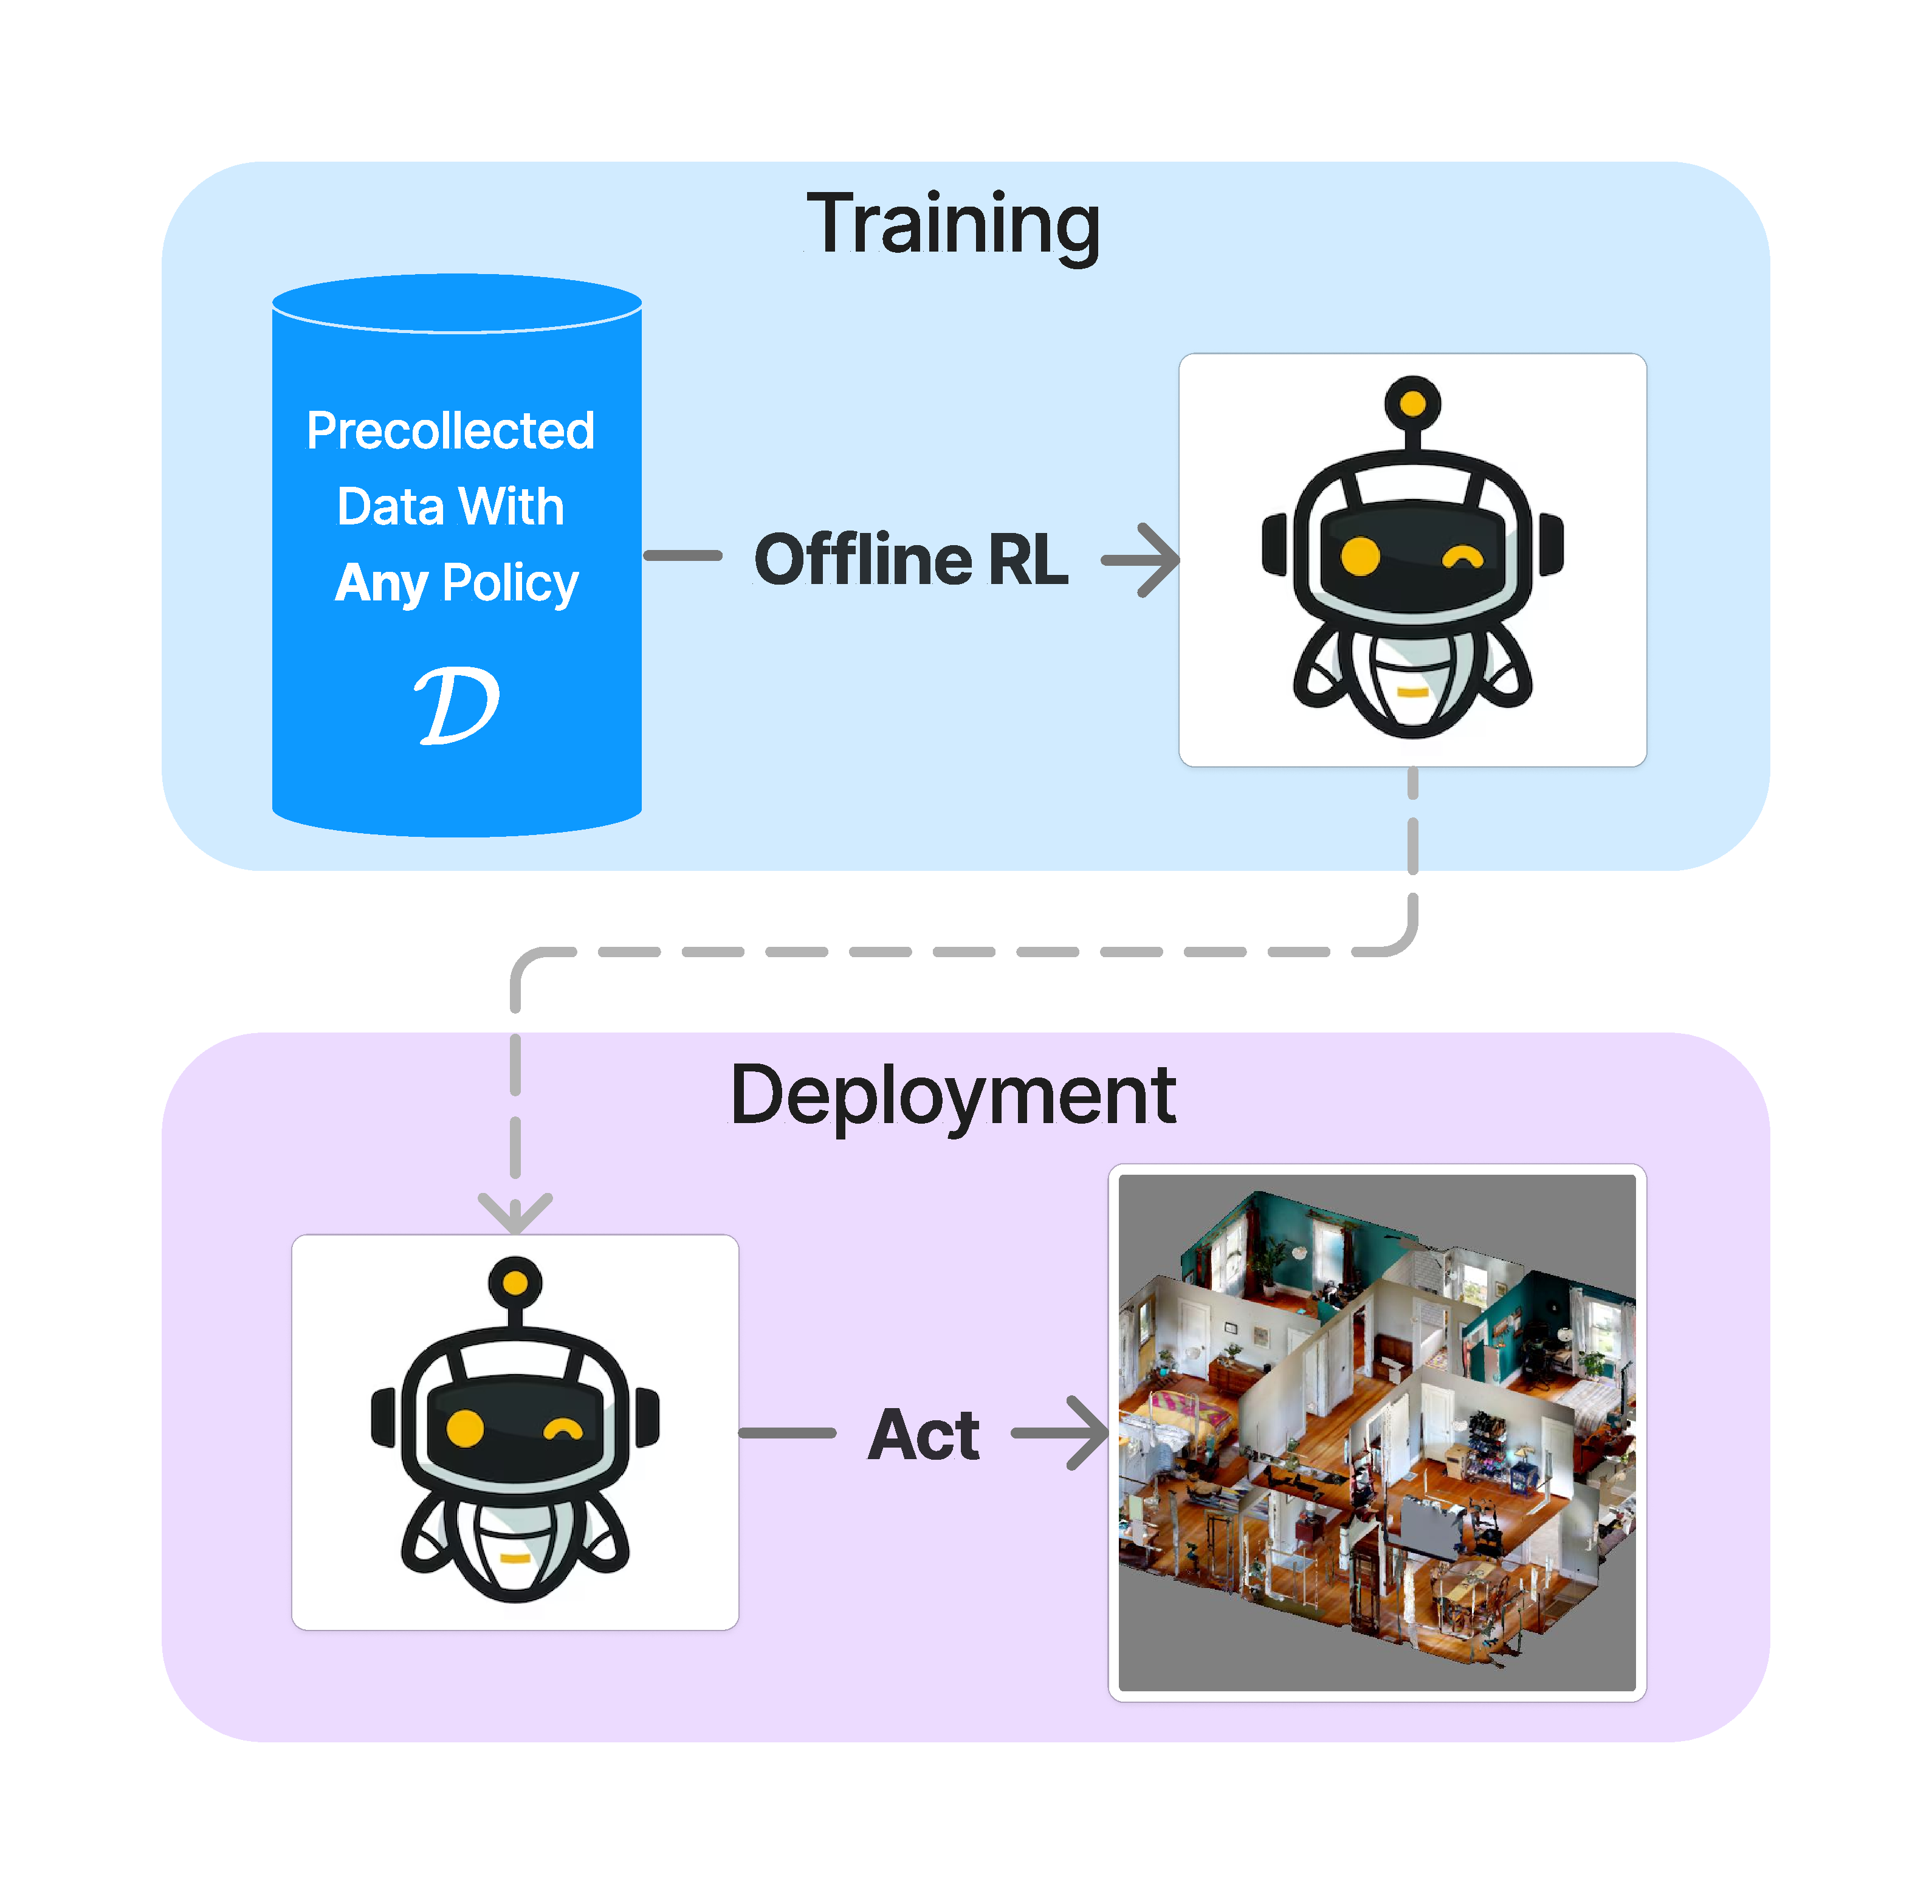
\includegraphics[width=.8\linewidth]{figures/offnav/graphical_abstract}
    \caption{
    By leveraging on the offline reinforcement learning paradigm, we can train agents from a fixed dataset of navigation experience, without querying any environment.
    This opens the possibility to create many navigation datasets from any navigation agent in any \textbf{real or simulated} environment, and then use them to train new agents for different scenarios without the need to ever query that environment.
    }
    \label{fig:abstract_offnav}
\end{figure}

%Current state-of-the-art models~\cite{ramrakhya2023} achieve 70,4\% SR on Habitat Simulator~\cite{szot2021} by using a two-phase training schedule.
%First, a


%% Maybe for experiments
%If the agent successfully reaches the object within a time limit, the episode is considered successful.
%In the other case, it is considered a failure.
%The performance of the navigation is measured by averaging the success over all the episodes present in an evaluation, and it receives the name of Success Rate (SR).
%%%%%%%%%%%%%%%%%%%%%%%%%%%

\subsection{Offline Visual Semantic Navigation}\label{subsec:offline-navigation}

In this work, we study \acrshort{objnav} navigation~\cite{batra2020}, a setup in which an agent is asked to navigate to a target object in an environment.
To perform this task, the agent does it using only egocentric perceptions.
Specifically, the agent receives RGB images and GPS+Compass information that provides the agent with the current position and orientation relative to the starting point.
The set of movements is discrete and consists of the following actions: \turnleft, \turnright, \moveforward, \lookup, \lookdown and \stopac.
If the agent spawns the \stopac action within 1$m$ Euclidean distance respect to the target object within a 500 steps time limit, the episode is considered successful.
In the other case, it is considered a failure.
The success rate (SR) is measured by averaging the success over all the episodes present in an evaluation set.
%We also report the Success weighted by Path Length (SPL) metric, which is the success rate weighted by the ratio between ideal and actual path length.

Since we are on an offline RL setup, we need a previously collected dataset of navigation experience.
The dataset that we chose is collected in~\cite{ramrakhya2023}.
It consists of $77k$ episodes of human navigation trajectories using the HM3D~\cite{Ramakrishnan2021HabitatMatterport3D} dataset.

We train our policies using our DD-IQL implementation on the human demonstrations.
The objetive is to find a policy with optimal parameters $\phi^*$ that maximizes the expected return from the dataset.
To do so, the IQL algorithm relies on the use of expectile regression to modify a temporal-difference (TD) loss.
This modified TD loss is able to learn an approximate Q-function from the dataset actions.
This Q-function does not explicitly represent the corresponding policy, so a separate policy extraction step is needed.
For policy extraction, we use advantage-weighted regression~\cite{peters2007, peng2019advantageweighted}:

\begin{equation}
    L_\pi(\phi)=\mathbb{E}_{(s, a) \sim \mathcal{D}}\left[\exp \left(\beta\left(Q_{\hat{\theta}}(s, a)-V_\psi(s)\right)\right) \log \pi_\phi(a|s)\right]\; ,
    \label{eq:loss}
\end{equation}

where $\beta \in [0, \infty)$ controls the trade-off between cloning the expert policy and maximizing the Q-function.
This loss can be seen as a selection of most optimal actions to clone in the dataset.
We also employ inflection weighting~\cite{wijmans2019} to modify the loss function, thereby giving more importance to those time steps where there is a change in actions.

For the policy architecture, we use a simple CNN+RNN model from\cite{ramrakhya2023}.
The difference is that we use ResNet18 for the visual encoders.
We copy the same architecture for the policy net, the Q net and the Q target net.
For the V net, we only use the visual encoder and a single linear layer, without any recurrent module.

\subsection{Experiments and Results}\label{subsec:experiments_offnav}

Is an offline RL algorithm able to learn navigation policies effectively?
To answer this question, we have trained our DD-IQL model using the expert demonstrations on five different experimental setups.
These setups have been designed with an incremental difficulty.
The first three are evaluated on the same environments in which the agents were trained, while the last two are evaluated on different environments.
The details of the setups are depicted on figure~\ref{fig:setups}.

We compare our results with the current state-of-the-art model PirlNav~\cite{ramrakhya2023}.
This model is based on a two-phase training schedule.
The first phase is a supervised learning phase, where the model is trained using behavior cloning on the expert demonstrations.
The second phase is a reinforcement learning phase, where the model is fine-tuned using DD-PPO~algorithm~\cite{wijmans2020}.
For a fair comparison, we train the PirlNav agent using only the behavior cloning phase on the same setups as our OffNav model.

Results are shown on table~\ref{tab:success}.
It can be seen that both methods obtain similar performance on setups 1 to 3.
Offnav method outperforms PirlNav on setup 2, while PirlNav outperforms OffNav on setup 3, and both of them obtain 100\% SR on setup 1.
When evaluated on setup 4, PirlNav outperforms OffNav by 2.27\% absolute points.
However, on setup 5, the most challenging one, OffNav outperforms PirlNav by 8.69\% absolute points.


\begin{table}
    \centering
    \begin{tabular}{c|ccc}
        \toprule
        \textit{Experimental Setup} & \textit{OffNav}  & \textit{PirlNav} \\
        \midrule
        \textsc{Setup 1}            & 100\%          & 100\%   \\
        \textsc{Setup 2}            & \textbf{79.31\%} & 72.50\%          \\
        \textsc{Setup 3}            & 75.78\%          & \textbf{77.63\%} \\
        \textsc{Setup 4}            & 25.00\%          & \textbf{27.27\%} \\
        \textsc{Setup 5}            & \textbf{34.78\%} & 26.09\%          \\
        \bottomrule
    \end{tabular}
    \caption{Success Rate for OffNav and PirlNav methods on the five experimental setups.}
    \label{tab:success}
\end{table}

\begin{figure}
    \centering
    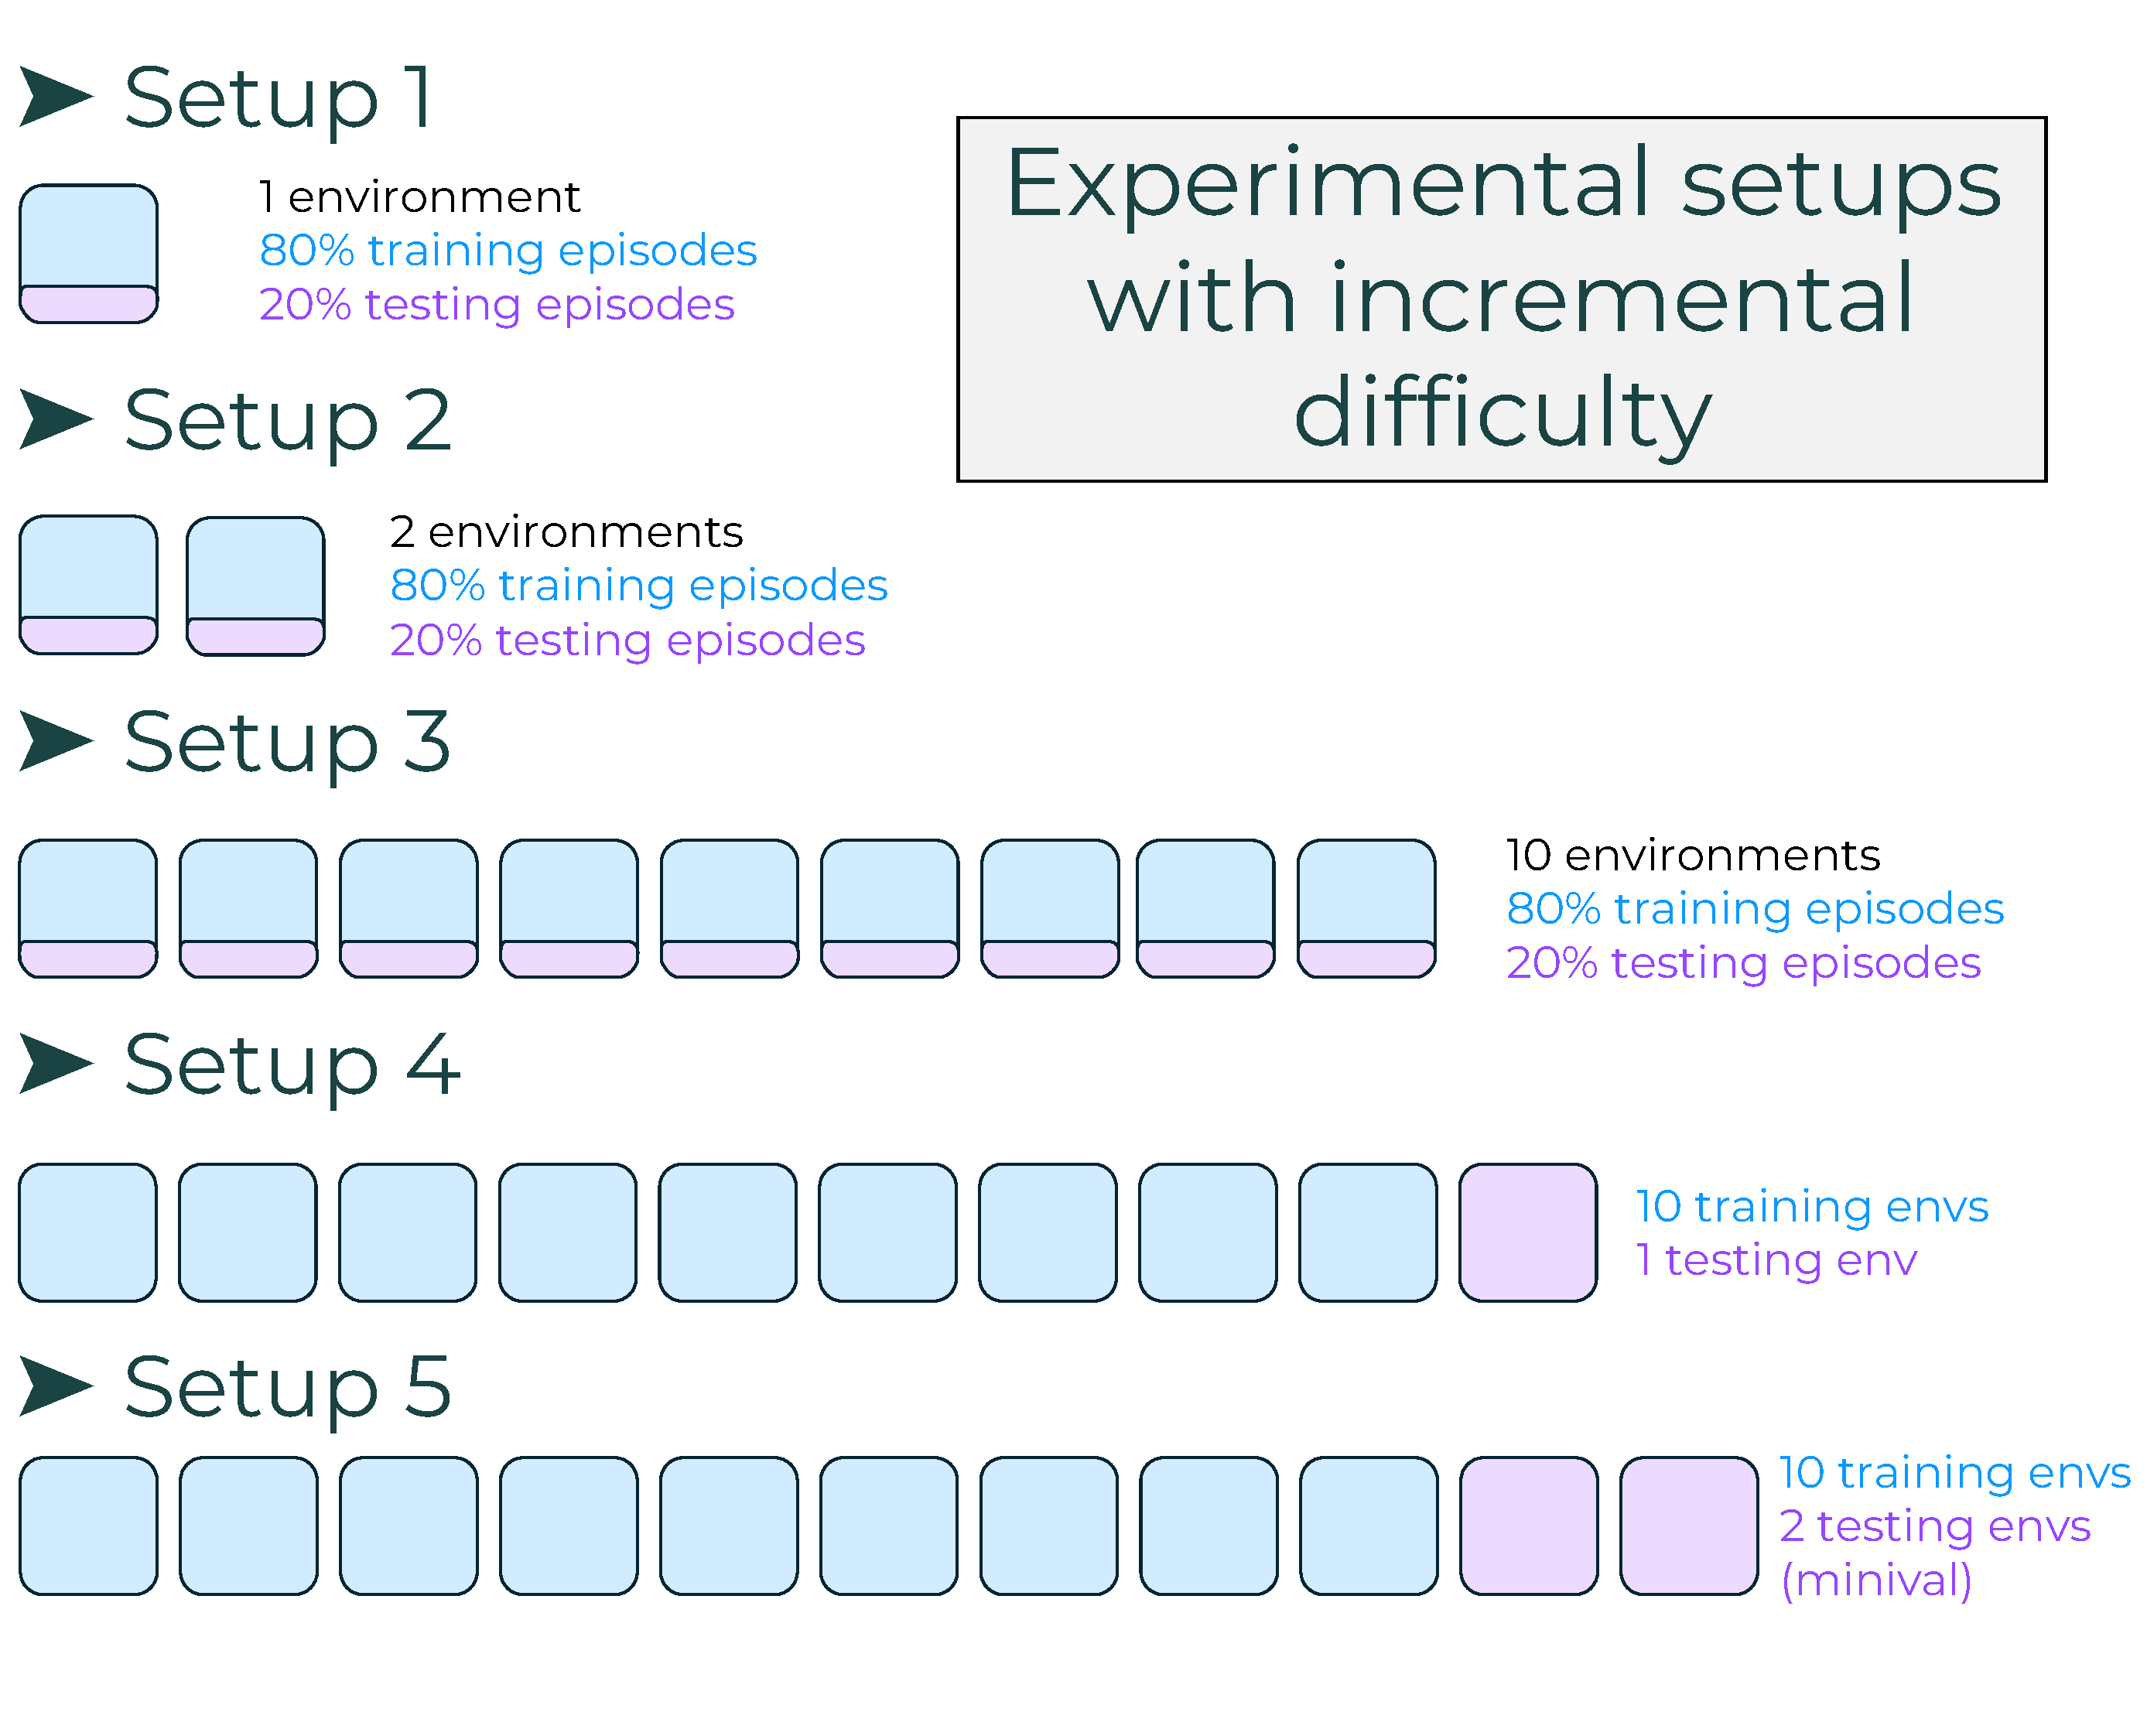
\includegraphics[width=\linewidth]{figures/offnav/experimental_setups}
    \caption{Five experimental setups designed with an incremental difficulty.}
    \label{fig:setups}
\end{figure}

\subsection{Conclusions and Future Work}\label{subsec:conclusions_offnav}

From the results obtained in the experiments, we can conclude that the proposed OffNav method is able to learn navigation policies effectively from human demonstrations.
It can also be seen that the method is able to generalize to unseen environments, as shown in setups 4 and 5, and outperform the state-of-the-art model PirlNav~\cite{ramrakhya2023} in the most challenging one.
Future work will focus on training the policy with more diverse environments to improve its generalization capabilities and further extend this analysis.

\section{Meta Imitation Learning for Real World Navigation}\label{sec:mil-for-real-world-navigation}

\subsection{Introduction}\label{subsec:introduction_metanav}

Training reinforcement learning algorithms for specific tasks has been a common practice in the field of robotics.


\subsection{Meta Imitation Learning for Robotic Visual Navigation}\label{subsec:meta-imitation-learning-for-robotic-visual-navigation}

\subsection{Experiments}\label{subsec:experiments_metanav}

\begin{table}[t]
    \centering
    \begin{tabular}{c|cccc}
        \toprule
        \textit{\textbf{Setup}} & \textit{\textbf{SR ($\uparrow$)}} & \textbf{\textit{SPL ($\uparrow$)}} & \textit{\textbf{Distance to Goal ($\downarrow$)}} \\ \midrule
        1                       & 89.18\%                           & 40.04\%                            & 0.29                                              \\
        2                       & 76.10\%                           & 33.92\%                            & 0.97                                              \\
        3                       & 64.19\%                           & 33.11\%                            & 1.99                                              \\
        4                       & 23.07\%                           & 11.87\%                            & 12.23                                             \\
        5                       & 21.74\%                           & 9.38\%                             & 7.99                                              \\
    \end{tabular}
    \caption{Evaluation of MetaNav on the \acrshort{vsn} task. Results obtained with continuos evaluation}
    \label{tab:metanav_continuos}
\end{table}


\begin{table}[t]
    \centering
    \begin{tabular}{c|cccc}
        \toprule
        \textit{\textbf{Setup}} & \textit{\textbf{SR ($\uparrow$)}} & \textbf{\textit{SPL ($\uparrow$)}} & \textit{\textbf{Distance to Goal ($\downarrow$)}} \\ \midrule
        1                       & 83.33\%                           & 40.04\%                            & 0.29                                              \\
        2                       & 60.78\%                           & 26.58\%                            & 1.74                                              \\
        3                       & 55.19\%                           & 26.21\%                            & 2.54                                              \\
        4                       & 16.67\%                           & 4.84\%                             & 12.72                                             \\
        5                       & 25.00\%                           & 9.31\%                             & 8.19                                              \\
    \end{tabular}
    \caption{Evaluation of MetaNav on the \acrshort{vsn} task. Results obtained with per episode evaluation}
    \label{tab:metanav_episode}
\end{table}

\subsection{Conclusions}\label{subsec:conclusions_metanav}